% -*- latex -*-
%
% The SAND document class is maintained at:
%
%    http://www.cs.sandia.gov/SANDreport/sandHome.html
%
% This page also as instructions and documentation on commands.
%
\documentclass[12pt,report]{SANDreport}

\SANDnum{SAND2013-xxxx}
\SANDprintDate{December 2013}

\title{A Pervasive Parallel Framework for Visualization: Final Report for
  FWP~10-014707}
\author{Kenneth~Moreland}
\SANDauthor{Kenneth~Moreland}
\date{} % Leave empty


\usepackage{amsfonts}
\usepackage{amssymb}
\usepackage{amsmath}
\usepackage{booktabs}
\usepackage{graphicx}
\usepackage{varioref}
\usepackage{fancyvrb}
\usepackage{ifthen}
\usepackage{cite}
\usepackage{subfig}
\usepackage{xspace}

\usepackage{makeidx}
\makeindex

\usepackage[pdfborder={0 0 0}]{hyperref}
\usepackage{verbatim}

\usepackage{color}
\definecolor{yellow}{rgb}{1,1,0}
\definecolor{black}{rgb}{0,0,0}
\definecolor{ltcyan}{rgb}{.75,1,1}
\definecolor{red}{rgb}{1,0,0}
\definecolor{gray}{rgb}{.6,.6,.6}
\definecolor{darkred}{rgb}{0.5,0,0}
\definecolor{darkgreen}{rgb}{0,0.5,0}

\usepackage{listings}
\lstloadlanguages{C,C++}
\lstset{fontadjust=false,basicstyle=\scriptsize\ttfamily}
%% \lstset{numbers=left, numberstyle=\tiny, stepnumber=1, numbersep=2pt}
\lstdefinelanguage{Dax}{
  morekeywords={struct,class,public,typedef, void, template, return, operator, const, for, int},
  morekeywords={[2]DAX_CONT_EXPORT,DAX_EXEC_EXPORT,DAX_EXEC_CONT_EXPORT,
                   _1,_2,_3,_4, In, Out, Point, Field, Topology,
                   Id, Id3, Tuple, Vector2,Vector3,Vector4,
                   WorkletMapField, WorkletMapCell,
                   ParametricCoordinates, CellDerivative},
  morekeywords={[3]dax,exec,cont,math},
  morekeywords={[4]ControlSignature, ExecutionSignature}
}
\lstset{language=Dax}
\lstset{
  keywordstyle=[2]\color{blue},
  keywordstyle=[3]\color{darkred},
  keywordstyle=[4]\color{darkgreen}
}

% Cite commands I use to abstract away the different ways to reference an
% entry in the bibliography (superscripts, numbers, dates, or author
% abbreviations).  \scite is a short cite that is used immediately after
% when the authors are mentioned.  \lcite is a full citation that is used
% anywhere.  Both should be used right next to the text being cited without
% any spacing.
\newcommand*{\lcite}[1]{~\cite{#1}}
\newcommand*{\scite}[1]{~\cite{#1}}

\newcommand{\etal}{et al.}

\newcommand*{\keyterm}[1]{\emph{#1}}

\newcommand{\fix}[1]{{\color{red}\textsc{[#1]}}}

% Avoid putting figures on their own page.
\renewcommand{\textfraction}{0.05}
\renewcommand{\topfraction}{0.95}
\renewcommand{\bottomfraction}{0.95}

% Make sure this is big enough so that only big figures end up on their own
% page but small enough so that if a figure does have to be on its own
% page, it won't push everything to the bottom because it's not big enough
% to have its own page.
\renewcommand{\floatpagefraction}{.75}

\begin{document}

\maketitle

\begin{abstract}
  \fix{Add abstract}
\end{abstract}

\clearpage

\chapter*{Acknowledgement}

\fix{Add thanks and funding statements.}

\cleardoublepage % TOC should start on an odd page
\tableofcontents
\listoffigures
\listoftables

\clearpage

\chapter*{Executive Summary}
\addcontentsline{toc}{chapter}{Executive Summary}

% -*- latex -*-

The evolution of the computing world from teraflop to petaflop has been
relatively effortless, with several of the existing programming models
scaling effectively to the petascale. The migration to exascale, however,
poses considerable challenges. All industry trends infer that the exascale
machine will be built using processors containing hundreds to thousands of
cores per chip. It can be inferred that efficient concurrency on exascale
machines requires a massive amount of concurrent threads, each performing
many operations on a localized piece of data.

Currently, visualization libraries and applications are based off what is
known as the visualization pipeline. In the pipeline model, algorithms are
encapsulated as \keyterm{filters} with inputs and outputs. These filters
are connected by setting the output of one component to the input of
another. Parallelism in the visualization pipeline is achieved by
replicating the pipeline for each processing thread. This works well for
today's distributed memory parallel computers but cannot be sustained when
operating on processors with thousands of cores.

Our project investigates a new visualization framework designed to exhibit
the pervasive parallelism necessary for extreme scale machines. Our
framework achieves this by defining algorithms in terms of
\keyterm{worklets}\index{worklet}, which are localized stateless
operations. Worklets are atomic operations that execute when invoked unlike
filters, which execute when a pipeline request occurs. The worklet design
allows execution on a massive amount of lightweight threads with minimal
overhead. Only with such fine-grained parallelism can we hope to fill the
billions of threads we expect will be necessary for efficient computation
on an exascale machine.


\section*{Progress and Accomplishments}
\addcontentsline{toc}{section}{Progress and Accomplishments}

Although the ``Pervasive Parallel Processing Framework for Data
Visualization and Analysis at Extreme Scale'' project is a research project
to make progress on designing and implementing massively threaded
visualization algorithms, our project also aims to explore techniques that
simplify the development of such algorithms and to provide useful software
for this purpose. To that end we have developed the Dax toolkit as a
deployment platform for our research. The Dax toolkit is a comprehensive
C++ header library that embodies the techniques developed within the
project. A summary of our major accomplishments is as follows.

\paragraph*{Development of Framework}

Much thought has gone into the design of the core components of the toolkit
API that users will use to define their analysis algorithms. The API has
been developed to be succinct, type safe, and efficient when executing on
multiple architectures. We developed adapters to enable execution and
testing of the framework on multiple architectures including GPUs and
CPUs. We added support for advanced core data structures needed for data
analysis such as data set types, cell types, and structures for sorting
geometrical and topological information. The framework supports advanced
analysis algorithms including those that change both geometry and topology,
such as marching cubes and threshold.
  
We reevaluated the use of pipelines for analysis on massively parallel
architectures. The idea being that the framework would control the flow of
execution and perform a limited sort of kernel fusion to maximize the
amount of computation per data load. We concluded that the complexity in
API and the toolkit implementation due to scheduling and execution of
pipelines could be greatly simplified by abandoning the connected pipeline
paradigm. Instead, the users directly manage the data flow by dispatching
calls to analysis worklets in order. We find that the framework structure
lends to developing in such a way as to encourage performing as many
operations per data load as possible without further adjustment by the
framework.

\paragraph*{Cross-Platform Analysis}

Our implementation now supports multiple target platforms including GPU
(using CUDA\lcite{CUDA} via Thrust\lcite{Thrust}), multi-core CPUs (using
either OpenMP\lcite{OpenMP} via Thrust or TBB\lcite{TBB}), and single core
CPU. We achieve these cross-platform implementations through careful
structure of the toolkit code. We have identified the basic features
specific to each multithreaded device and encapsulated them in a unit
called a \index{device~adapter}\keyterm{device adapter}. A device adapter
can be implemented by providing only a thread scheduling mechanism although
more efficient custom algorithms can be provided as well. A device adapter
can be changed with a single template parameter, thus enabling the porting
of the majority of code with very little development.

\paragraph*{Development of Analysis Algorithms}

We developed infrastructure to support analysis algorithms including those
that change topology and geometry. These algorithms require multiple
passes, particularly on architectures with memory restrictions, such as
GPUs and potentially proposed exascale machines. With the framework API and
infrastructure matured we developed key analysis algorithms that also
exercise the framework. These include thresholding of cells using point
fields, marching cubes for generating isosurfaces, and computing derived
fields.

\paragraph*{Software Infrastructure}

For software reliability and correctness, we set up a software process
including a testing framework, dashboards for daily regression testing and
verification, a developer wiki for design and implementation discussions,
doxygen for API documentation, and mailing list for developer
communication.


\section*{Presentations and Publications}
\addcontentsline{toc}{section}{Presentations and Publications}

During the course of our project, we presented our work to a broad audience
to gain feedback and discuss the vision we have for parallelizing
visualization algorithms. Some of the major locations where we presented
the Dax toolkit are:

\begin{description}
  \raggedright
\item\textbf{Dax: Data Analysis at Extreme,} paper by Kenneth Moreland,
  Utkarsh Ayachit, Berk Geveci, and Kwan-Liu Ma. In Proceedings of SciDAC
  2011, July 2011.
\item\textbf{Dax Toolkit: A Proposed Framework for Data Analysis and
  Visualization at Extreme Scale,} paper by Kenneth Moreland, Utkarsh
  Ayachit, Berk Geveci, and Kwan-Liu Ma. In IEEE Symposium on Large-Scale
  Data Analysis and Visualization (LDAV), October 2011.
\item\textbf{Next-Generation Capabilities for Large-Scale Scientific
  Visualization,} presentation by Kenneth Moreland. 15th SIAN Conference on
  Parallel Processing for Scientific Computing, February 2012.
\item\textbf{Next-Generation Codes/Portability: Dax Perspective,}
  presentation by Kenneth Moreland, DOECGF, April 2012.
\item\textbf{Oh, \$\#*@! Exascale! The Effect of Emerging Architectures on
  Scientific Discovery,} paper by Kenneth Moreland. In 2012 SC Companion
  (Proceedings of the Ultrascale Visualization Workshop), November 2012,
  pg. 224-231. DOI 10.1109/SC.Companion.2012.38.
\item\textbf{Dax for Multi- and Many-Core Architectures,} panel
  presentation by Kenneth Moreland. Supercomputing, November 2012.
\item\textbf{The SDAV Software Frameworks for Visualization and Analysis on
  Next-Generation Multi-Core and Many-Core Architectures,} paper by
  Christopher Sewell, Jeremy Meredith, Kenneth Moreland, Tom Peterka, Dave
  DeMarle, La-ta Lo, James Ahrens, Robert Maynard, and Berk Geveci. In 2012
  SC Companion (Proceedings of the Ultrascale Visualization Workshop),
  November 2012, pg. 206-214. DOI 10.1109/SC.Companion.2012.36.
\item\textbf{Flexible Analysis Software for Emerging Architectures,} paper
  by Kenneth Moreland, Brad King, Robert Maynard, and Kwan-Liu Ma. In 2012
  SC Companion (Proceedings of Petascale Data Analytics: Challenges and
  Opportunities), November 2012. DOI 10.1109/SC.Companion.2012.115.
\item\textbf{Optimizing Threshold for Extreme Scale Analysis,} poster by
  Robert Maynard, Kenneth Moreland, Utkarsh Ayachit, Berk Geveci, and
  Kwan-Liu Ma. In Proceedings of SPIE Visualization and Data Analysis,
  February 2013.
\item\textbf{A Survey of Visualization Pipelines,} paper by Kenneth
  Moreland. IEEE Transactions on Visualization and Computer Graphics,
  19(3), March 2013. DOI 10.1109/TVCG.2012.133.
\item\textbf{DaxToolkit: Efficient Visualization at Extreme Scale,}
  presentation by Robert Maynard, GPU Technology Conference, March 2013.
\item\textbf{The effect of emerging architectures on data analysis
  software,} panel presentation by Kenneth Moreland, SOS 17, March 2013.
\item\textbf{Dax,} presentation by Kenneth Moreland, DOECGF, April 2013.
\item\textbf{Research Challenges for Visualization Software,} paper by Hank
  Childs, Berk Geveci, Will Schroeder, Jeremy Meredith, Kenneth Moreland,
  Christopher Sewell, Torsten Kuhlen, and E. Wes Bethel. IEEE Computer,
  46(5), May 2013, pg. 34-42. DOI 10.1109/MC.2013.179.
\item\textbf{Upcoming Challenges for Scientific Visualization Software:
  Programming Future Architectures,} panel presentation by Kenneth
  Moreland, IEEE Visualization, October 2013.
\item\textbf{A Classification of Scientific Visualization Algorithms for
  Massive Threading,} paper by Kenneth Moreland, Berk Geveci, Kwan-Liu Ma,
  and Robert Maynard. In Proceedings of the Ultrascale Visualization
  Workshop, November 2013. DOI 10.1145/2535571.2535591.
\end{description}


\SANDmain % Start the main part of the document.

\chapter{Introduction}
\label{chap:Introduction}

% -*- latex -*-

High-performance computing relies on ever finer threading. Recent advances
in processor technology include greater numbers of cores, hyperthreading,
and accelerators with integrated blocks of cores, all of which require more
software parallelism to achieve peak performance. Current visualization
solutions cannot support this extreme level of concurrency. Extreme scale
systems require a new programming model and a fundamental change in how we
design algorithms. This document is a report on the project titled ``A
Pervasive Parallel Processing Framework for Data Visualization and Analysis
at Extreme Scale'' funded by the ASCR Scientific Data Management and
Analysis at Extreme Scale program. This project delivers its work with the
creation of the Data Analysis at Extreme (Dax) toolkit.

The Dax toolkit supports a number of algorithms and the ability to design
further algorithms through a top-down design with an emphasis on extreme
parallelism. Dax also provides support for finding and building links
across topologies, making it possible to perform operations that determine
manifold surfaces, interpolate generated values, and find
adjacencies. Although Dax provides a simplified high-level interface for
programming, its template-based code removes the overhead of abstraction.

\begin{figure}
\centering
\begin{tabular}{cc}
\begin{lstlisting}
int vtkCellDerivatives::RequestData(...)
{
  ...[allocate output arrays]...
  ...[validate inputs]...




  for (cellId=0;
       cellId < numCells;
       cellId++)
    {
    ...[update progress]...
    input->GetCell(cellId, cell);
    inScalars->GetTuples(cell->PointIds,
                         cellScalars);
    scalars = cellScalars->GetPointer(0);

    subId =
      cell->GetParametricCenter(pcoords);


    cell->Derivatives(
      subId, pcoords, scalars, 1, derivs);
 
    outGradients->SetTuple(cellId,derivs);

    }
  ...[cleanup]...
}
\end{lstlisting}
&
\begin{lstlisting}
struct CellGradient
  : public dax::exec::WorkletMapCell
{
  typedef void ControlSignature(
      Topology, Field(Point),
      Field(Point), Field(Out));
  typedef _4 ExecutionSignature(_1,_2,_3);
 
  template<class CellTag>
  DAX_EXEC_EXPORT
  dax::Vector3 operator()(...)
  {






    dax::Vector3 parametricCellCenter =
        dax::exec::ParametricCoordinates<
          CellTag>::Center();
 
    return dax::exec::CellDerivative(
        parametricCellCenter,
        coords,
        pointField,
        cellTag);
  }
 
};
\end{lstlisting}
\\
VTK Code & Dax Code
\end{tabular}
\caption[Comparison of VTK code and Dax code.]{A comparison of code to
  compute a localized field derivative within VTK and within the Dax
  toolkit.}
\label{fig:CompareVTKDax}
\end{figure}

The Dax toolkit simplifies the development of parallel visualization
algorithms. Consider the code samples in Figure~\ref{fig:CompareVTKDax}
that come from the Visualization Toolkit (VTK) on the left and our Dax
toolkit on the right. Both implementations perform the same operation; they
estimate gradients using finite differences. Both toolkits provide similar
classes and functions, and consequently the code looks remarkably similar.

However, because the Dax toolkit is structured such that it can schedule
its execution on a GPU, we measure that it performs this operation over 100
times faster than the VTK code running on a single CPU. Furthermore, the
Dax API can be switched to a different device by changing only a single
line of code. Dax currently provides scheduling for CUDA (GPU), OpenMP
(multi-core CPU), Intel Threading Building Blocks (multi-core CPU), and
serial execution.

This report documents the design of the Dax
toolkit. Chapter~\ref{chap:Overview} provides an overview of the Dax
toolkit and describes the higher level
context. Chapter~\ref{chap:Documentation} describes the API of the Dax
toolkit and provides the initial software
documentation. Chapter~\ref{chap:ProgressReport} reports on further lessons
and achievements attained during this project.


\chapter{Overview of Dax Toolkit}
\label{chap:Overview}

% -*- latex -*-

\section{General Approach}
\label{sec:GeneralApproach}

\fix{-Philosophy of algorithm design}

\fix{--Characterize algorithms by local operations}

\fix{--Safely encapsulate algorithms in ``worklets''}

\fix{---Better programming through constraints}

\fix{--Make resuable components for ``communicative'' operations}


\section{Structure of Dax Framework}
\label{sec:StructureOfDaxFramework}

\fix{Picture of cont/exec/d adapter/worklet}


\section{Device Independence}
\label{sec:DeviceIndependence}

\fix{Device adapter section of PDAC2012 paper.}

\fix{Reference to Section~\ref{sec:DeviceAdapterAlgorithms}. Also need to
  talk about execution array management.}


\section{Generic Memory Structures}
\label{sec:GenericMemoryStructures}

\fix{Generic array handle section of PDAC2012 paper.}

\fix{Reference to Section~\ref{sec:ArrayHandle}.}

\section{Generic Scheduling}
\label{sec:GenericScheduling}

\fix{Schedule metaprograms section of PDAC2012 paper.}

\fix{Reference to Section~\ref{sec:Scheduling}.}


\chapter{Dax Toolkit Documentation}
\label{chap:Documentation}

% -*- latex -*-

This chapter documents the implementation and API of the Dax toolkit. This
documentation is primarily in reference to users of the Dax toolkit but
also gives some details on the internal implementation.

The Dax toolkit is written in C++ and makes extensive use of templates. The
toolkit is implemented as a header library, meaning that all the code is
implemented in header files (with extension \textfilename{.h}) and
completely included in any code that uses it. This is typically necessary
of template libraries, which need to be compiled with template parameters
that are not known until they are used. This also provides the convienience
of allowing the compiler to inline user code for better performance.

When documenting the Dax API, the following conventions are used.
\begin{itemize}
\item Filenames are printed in a \textfilename{sans serif font}.
\item C++ code is printed in a \textcode{monospace font}.
\item Macros and namespaces from the Dax toolkit are printed
  in \textnamespace{red}.
\item Identifiers from the Dax toolkit are printed in
  \textidentifier{blue}.
\item Signatures, described in Section~\ref{sec:GenericScheduling}, are
  printed in \textsignature{green}.
\end{itemize}

\section{Package Structure}
\label{sec:PackageStructure}

\index{packages|seealso{namespace}}
\index{packages|(}

The Dax toolkit is organized in a hierarchy of nested packages. The Dax
toolkit places definitions in \keyterm{namespaces} \index{namespace} that
correspond to the package (with the exception that one package may
specialized a template defined in a different namespace). Hence, the
description and

The base package is named \dax{}. All classes within the Dax toolkit are
placed either directly in the \dax{} package or in a package beneath
it. This helps prevent name collisions between the Dax toolkit and any
other library.

As described in Section~\ref{sec:StructureOfDaxFramework}, the Dax API is
divided into two distinct environments: \index{environments} the control
environment \index{control~environment} and the execution
environment. \index{execution~environment} The API for these two
environments are located in the \daxcont{} and \daxexec{} packages,
respectively. Items located in the base \dax{} namespace are available in
both environments.

Although it is conventional to spell out names in identifiers (see the
coding conventions in Section~\ref{sec:CodingConventions}), there is an
exception to abbreviate control and execution to \textnamespace{cont}
and \textnamespace{exec}, respectively. This is because it is also part of
the coding convention to declare the entire namespace when using an
identifier that is part of the corresponding package. The shorter names
make the identifiers easier to read, faster to type, and more feasible to
pack lines in 80 column displays. These abbreviations are also used instead
of more common abbreviations (e.g. ctrl for control) because, as part of
actual English words, they are easier to type.

Worklets provided by the Dax toolkit, described in
Section~\ref{sec:ProvidedWorklets}, are contained in the \daxworklet{}
package. Although the operation of a worklet happens exclusively in the
execution environment, worklets are typically initialized in the control
environment. Thus, the \daxworklet{} package is not encapsulated in either
\daxcont{} or \daxexec{}.

The Dax toolkit provides a base set of library functions that are ported to
the various systems and compilers on which it is used. These functions are
located in the \daxmath{} package. The features in \daxmath{} are available
in both the control and execution environments, but they are typically used
in the execution environment.

The Dax toolkit contains code that uses specalized compiler features, such
as those with CUDA and OpenMP, or libraries, such as Intel Threading
Building Blocks, that will not be available on all machines. Code for these
features are encapsulated in their own packages: \daxcuda{}, \daxopenmp{},
and \daxtbb{}. Within each one of these packages, there will
be \textnamespace{cont} and \textnamespace{exec} namespaces as necessary to
denote features that are accessible in only one environment or the other.

The Dax toolkit contains OpenGL interoperability \index{OpenGL}
\index{interoperability} that allows data generated with Dax to be
efficiently transfered to OpenGL objects. This feature is encapsulated in
the \daxopengl{} package.

Figure~\ref{fig:Packages} provides a diagram of the Dax package hierarchy.

\begin{figure}
  \centering
  %% \begin{itemizetight}
  %% \item \textnamespace{dax}
  %%   \begin{itemizetight}
  %%   \item \textnamespace{cont}
  %%   \item \textnamespace{exec}
  %%   \item \textnamespace{worklet}
  %%   \item \textnamespace{math}
  %%   \item \textnamespace{cuda}
  %%     \begin{itemizetight}
  %%     \item \textnamespace{cont}
  %%     \end{itemizetight}
  %%   \item \textnamespace{openmp}
  %%     \begin{itemizetight}
  %%     \item \textnamespace{cont}
  %%     \end{itemizetight}
  %%   \item \textnamespace{tbb}
  %%     \begin{itemizetight}
  %%     \item \textnamespace{cont}
  %%     \end{itemizetight}
  %%   \item \textnamespace{opengl}
  %%   \end{itemizetight}
  %% \end{itemizetight}
  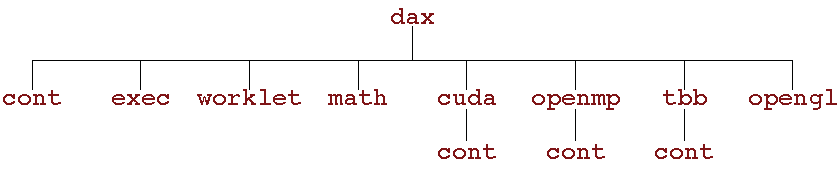
\includegraphics{images/PackageHierarchy}
  \caption{Dax package hierarchy.}
  \label{fig:Packages}
\end{figure}

By convention all classes will be defined in a file with the same name as
the class name (with a \textfilename{.h} extension) located in a directory
corresponding to the package name. For example, the \daxcont{ArrayHandle}
class is found in the \daxheader{dax/cont}{ArrayHandle.h} header. There
are, however, exceptions to this rule. Some smaller classes and types are
grouped together for convienience. These exceptions will be noted as
necessary.

Within each namespace there may also
be \textnamespace{internal}\indexnamespaceone{internal}
and \textnamespace{detail}\indexnamespaceone{detail}
sub-namespaces. The \textnamespace{internal} namespaces contain features
that are used internally and may change without
notice. The \textnamespace{detail} namespaces contain features that are
used by a particular class but must be declared outside of that
class. Users should generally ignore classes in these namespaces.

\index{packages|)}


\section{Basic Provisions}
\label{sec:BasicProvisions}

This section describes the core facilities provided by the Dax
toolkit. These include macros, types, and classes that define the
environment in which code is run, the core types of data stored, and
template introspection.

\subsection{Function and Method Exports}
\label{sec:FunctionAndMethodExports}

Any function or method defined by the Dax toolkit must come with an export
modifier that determines in which environments the function may be
run. These export modifiers are C macros that Dax uses to instruct the
compiler for which architectures to compile each method. Most user code
outside of the Dax toolkit need not use these macros with the important
exception of any classes passed to the Dax toolkit. This occurs when
defining new worklets, array containers, and device adapters.

Dax provides three export macros, \daxcontexport, \daxexecexport, and
\daxexeccontexport, which are used to declare functions and methods that
can run in the control environment, export environment, and both
environments, respectively. These macros get defined by including just
about any Dax header file, but including \daxheader{dax}{Types.h} will
ensure they are defined. 

The export macro is place after the template declaration, if there is one,
and before the return type for the function. Here is a simple example of a
function that will square a value. Since most types you would use this
function on have operators in both the control and execution environments,
the function is exported to both places.

\begin{daxexample}{Usage of export macro.}
template<class ValueType>
DAX_EXEC_CONT_EXPORT
ValueType Square(const ValueType &inValue)
{
 return inValue * inValue;
}
\end{daxexample}

The primary function of the export macros is to interject compiler-specific
keywords that specify what architecture to compile code for. For example,
when compiling with CUDA\index{CUDA}, the control exports have
\textcode{\_\_host\_\_} in them and execution exports have
\textcode{\_\_device\_\_} in them.

There is one additional export macro that is not used for functions but
rather used when declaring a constant data object that is used in the
execution environment. This macro is named
\daxmacro{DAX\_EXEC\_CONSTANT\_EXPORT}\index{export!constant}\index{constant~export}
and is used to declare a constant lookup table used when executing a
worklet. Its primary reason for existing is to add a
\textcode{\_\_constant\_\_} keyword when compiling with CUDA. This export
currently has no effect on any other compiler.

\subsection{Core Data Types}
\label{sec:CoreDataTypes}

Except in rare circumstances where precision is not a concern, the Dax
toolkit does not directly use the core C types like \textcode{int},
\textcode{float}, and \textcode{double}. Instead, Dax provides its own core
types, which are declared in \daxheader{dax}{Types.h}.

\subsubsection{Single Number Types}

All floating point values should be declared as type \dax{Scalar}, and all
integer values, generally used for indexing, should be declared as type
\dax{Id}. The chief advantage of using these declared types rather than the
core C types is that the precision can easily be changed. By default, both
types are 32 bits wide. The CMake configuration options
\cmakevar{DAX\_USE\_DOUBLE\_PRECISION} and \cmakevar{DAX\_USE\_64BIT\_IDS}
can be used to change the \dax{Scalar} type and \dax{Id} type,
respectively, to be 64 bits wide. The configuration can be overridden by
defining the C macro \daxmacro{DAX\_USE\_DOUBLE\_PRECISION} or
\daxmacro{DAX\_NO\_DOUBLE\_PRECISION} to force \dax{Scalar} to be either 64
or 32 bits and defining the C macro \daxmacro{DAX\_USE\_64BIT\_IDS} or
\daxmacro{DAX\_NO\_64BIT\_IDS} to force \dax{Id} to be either 64 or 32
bits. These macros must be defined before any Dax header files are included
to take effect. For convenience, you can include either
\daxheader{dax/internal}{ConfigureFor32.h} or
\daxheader{dax/internal}{ConfigureFor64.h} to force both \dax{Scalar} and
\dax{Id} to be 32 or 64 bits. The reason Dax uses macros to determine these
type widths rather than templates is to reduce the number of template
parameters required in the already template-heavy Dax classes and
functions.

\subsubsection{Vector Types}

Visualization algorithms also often require operations on short
vectors. Arrays indexed in up to three dimensions are common. Data is often
defined in 2-space and 3-space, and transformations are typically done in
homogeneous coordinates of length 4. To simplify these types of operations,
Dax provides several vector data types.

The types \dax{Id2} and \dax{Id3} are couple and triple values of type
\dax{Id}. The types \dax{Vector2}, \dax{Vector3}, and \dax{Vector4} are
couple, triple, and quadruple values of type \dax{Scalar}. The elements of
these vectors are accessed with the bracket operator, so they syntatically
appear like short arrays. They additionally have a constant named
\textidentifier{NUM\_COMPONENTS}\index{NUM\_COMPONENTS} to specify how many
components are in the tuple.

The default constructor of these vector types leaves the values
uninitialized. All vectors have a constructor with one arguments that is
used to initialize all components. All these vectors also have a
constructor that allows you to set the individual components. Likewise,
there are a set of \dax{make\_Id*} and \dax{make\_Vector*} functions that
build initialized vector types.

\begin{daxexample}{Creating vector types.}
dax::Vector3 A(1);                      // A is {1, 1, 1}
A[1] = 2;                               // A is now {1, 2, 1}
dax::Vector3 B(1, 2, 3);                // B is {1, 2, 3}
dax::Vector3 C = make_Vector3(3, 4, 5); // C is {3, 4, 5}
\end{daxexample}

The vector types all support component-wise arithmetic using the operators
for plus (\textcode{+}), minus (\textcode{-}), multiply (\textcode{*}), and
divide (\textcode{/}). They also support scalar to vector multiplication
with the multiply operator. The comparison operators equal (\textcode{==})
is true if every pair of corresponding components are true and not equal
(\textcode{!=}) is true otherwise.  A special \dax{dot} function is
overloaded to provide a dot product for every type of vector.

\begin{daxexample}{Vector operations.}
dax::Vector3 A(1, 2, 3);
dax::Vector3 B(4, 5, 6.5);
dax::Vector3 C = A + B;                     // C is {5, 7, 9.5}
dax::Vector3 D = 2 * C;                     // D is {10, 14, 19}
dax::Scalar s = dax::dot(A, B);             // s is 33.5
bool b1 = (A == B);                         // b1 is false
bool b2 = (A == dax::make_Vector3(1, 2, 3); // b2 is true
\end{daxexample}

\subsubsection{Tuple}

The Dax toolkit provides the templated class \dax{Tuple}\tparams{T,Size},
which is essentially a fixed length array of a given type. \dax{Tuple}
objects behave just like the vector types previously described but with any
type and length that you specify.

\begin{daxexample}{The tuple class.}
dax::Tuple<dax::Scalar, 5> A(2);  // A is {2, 2, 2, 2, 2}
for (int index = 1; index < NUM_COMPONENTS; index++)
  {
  A[index] = A[index-1] * 1.5;
  }
// A is now {2, 3, 4.5, 6.75, 10.125}
\end{daxexample}

The same operators that work on the vector types work on \dax{Tuple} with
the caveat that the operator must work on the component type of the
tuple. For example, the multiply operator will work fine on objects of type
\dax{Tuple}\tparams{char,3}, but the multiply operator will not work on objects
of type \dax{Tuple}\tparams{std::string,3} because you cannot multiply
objects of type \textcode{std::string}.

A \dax{Tuple} of the appropriate type can be used interchangeably with a
matching vector type. In fact, a vector type is really just a typedef over
a \dax{Tuple}. This is convienient for a number of things including writing
generic functions that work over all types.

\begin{daxexample}{Interchangeability of tuples and vector types.}
template<typename T, int Size>
DAX_EXEC_CONT_EXPORT
T SumComponents(const dax::Tuple<T,Size> &tuple)
{
  T result = tuple[0];
  for (int index = 1; index < Size; index++)
    {
    result += tuple[index];
    }
  return result;
}

void Foo()
{
  dax::Id a = SumComponents(dax::make_Id3(1, 2, 3));                    // a is 6
  dax::Scalar b = SumComponents(dax::make_Vector4(1.5, 2.5, 3.5, 4.5)); // b is 12
}
\end{daxexample}

In addition to generalizing vector operations and making arbitrarily long
vectors, \dax{Tuple} is useful for creating any sequence of homogeneous
objects. Here is a simple example of using \dax{Tuple} to hold the state of
a polygon.

\begin{daxexample}{Usage of a tuple.}
dax::Tuple<dax::Vector2,3> equilateralTriange(dax::make_Vector2(0.0, 0.0),
                                              dax::make_Vector2(1.0, 0.0),
                                              dax::make_Vector2(0.5, 0.866));
\end{daxexample}

\subsubsection{Pair}

The Dax toolkit defines a \dax{Pair}\tparams{T1,T2} templated object that
behaves just like \textcode{std:\colonhyp{}pair} from the standard template
library. The difference is that \dax{Pair} will work in both the execution
and control environment, whereas the STL \textcode{std::pair} does not
always work in the execution environment.

The Dax version of \dax{Pair} supports the same types, fields, and
operations as the STL version. Dax also provides a \dax{make\_Pair}
function for convenience.

\subsection{Traits}
\label{sec:Traits}

\index{traits|(}

When using templated types, it is often necessary to get information about
the type or specialize code based on general properties of the type. The
Dax toolkit uses traits classes to publish and retreive information about
types. A traits class is simply a templated structure that provides
typedefs for tag\index{tag} structures, empty types used for
identification. The traits classes might also contain constant numbers and
helpful static functions. See Mayers\scite{Mayers2009} for a description of
traits classes and their uses.

\subsubsection{Type Traits}

The \dax{TypeTraits}\tparams{T} templated class provides basic information
about a core type. These type traits are available for all the basic C++
types as well as the core Dax types described in
Section~\ref{sec:CoreDataTypes}. \dax{TypeTraits} contains the following
elements.

\begin{description}
\item[\textidentifier{NumericTag}] \index{NumericTag} This type is set to
  either \dax{TypeTraitsRealTag} or \dax{TypeTraitsIntegerTag} to signal
  that the type represents either floating point numbers or integers.
\item[\textidentifier{DimensionalityTag}] \index{DimensionalityTag} This
  type is set to either \dax{TypeTraitsScalarTag} or
  \dax{TypeTraitsVectorTag} to signal that the type represents either a
  single scalar value or a tuple of values.
\end{description}

The definition of \dax{TypeTraits} for \dax{Scalar} could like something
like this.
\begin{daxexample}{Definition of \protect \dax{TypeTraits}\tparams{\protect \dax{Scalar}}.}
namespace dax {

template<>
struct TypeTraits<dax::Scalar>
{
  typedef TypeTraitsRealTag NumericTag;
  typedef TypeTraitsScalarTag DimensionalityTag;
};

}
\end{daxexample}

Here is a simple example of using \dax{TypeTraits} to implement a generic
function that behaves like the modulus operator (\textcode{\%}) for all
types including floating points and vectors.

\begin{daxexample}[ex:TypeTraits]{Using \protect \dax{TypeTraits} for a generic modulus.}
#include <dax/TypeTraits.h>

template<typename T>
T Modulus(const T &numerator, const T &denominator);

namespace detail {

template<typename T>
T ModulusImpl(const T &numerator,
              const T &denominator,
              dax::TypeTraitsIntegerTag,
              dax::TypeTraitsScalarTag)
{
  return numerator % denominator;
}

template<typename T>
T ModulusImpl(const T &numerator,
              const T &denominator,
              dax::TypeTraitsRealTag,
              dax::TypeTraitsScalarTag)
{
  T quotient = numerator / denominator;
  return (quotient - dax::math::Floor(quotient))*demoninator;
}

template<typename T, typename NumericTag>
T ModulusImpl(const T &numerator,
              const T &denominator,
              NumericTag,
              dax::TypeTraitsVectorTag)
{
  T result;
  for (int componentIndex = 0; componentIndex < T::NUM_COMPONENTS; componentIndex++)
    {
    result[componentIndex] = Modulus(numerator[componentIndex],denominator[componentIndex]);
    }
}

} // namespace detail

template<typename T>
T Modulus(const T &numerator, const T &denominator)
{
  return detail::ModulusImpl(numerator,
                             denominator,
                             typename dax::TypeTraits<T>::NumericTag(),
                             typename dax::TypeTraits<T>::DimensionalityTag());
}
\end{daxexample}

\subsubsection{Vector Traits}

The \dax{VectorTraits}\tparams{T} templated class provides information and
accessors to vector and tuple types. It contains the following elements.

\begin{description}
\item[\textidentifier{ComponentType}] \index{ComponentType} This type is
  set to the type for each component in the vector. For example, a
  \dax{Vector3} has \textidentifier{ComponentType} defined as \dax{Scalar}.
\item[\textidentifier{NUM\_COMPONENTS}] \index{NUM\_COMPONENTS} An integer
  specifying how many components are contained in the vector.
\item[\textidentifier{HasMultipleComponents}] \index{HasMultipleComponents}
  This type is set to either \dax{VectorTraitsTagSingleComponent} if the
  vector length is size 1 or \dax{VectorTraitsTagMultipleComponents}
  otherwise. This tag can be useful for creating specialized functions when
  a vector is really just a scalar.
\item[\textcode{GetComponent}] \index{GetComponent} A static method that
  takes a vector and returns a particular component.
\item[\textcode{SetComponent}] \index{SetComponent} A static method that
  takes a vector and sets are particular component to a given value.
\item[\textcode{ToTuple}] \index{ToTuple} A static method that converts a
  vector of the given type to a \dax{Tuple}.
\end{description}

The definition of \dax{VectorTraits} for \dax{Id3} could like something
like this.
\begin{daxexample}{Definition of \protect \dax{VectorTraits}\tparams{\protect \dax{Id3}}.}
template<>
struct VectorTraits<dax::Id3>
{
  typedef dax::Id ComponentType;
  static const int NUM_COMPONENTS = 3;
  typedef VectorTraitsTagMultipleComponents HasMultipleComponents;

  DAX_EXEC_CONT_EXPORT
  static dax::Id &GetComponent(dax::Id3 &vector, int component) {
    return vector[component];
  }

  DAX_EXEC_CONT_EXPORT
  static void SetComponent(dax::Id3 &vector, int component, dax::Id value) {
    vector[component] = value;
  }

  DAX_EXEC_CONT_EXPORT
  static dax::Tuple<dax::Id,3> ToTuple(const dax::Id3 &vector) {
    return vector;
  }
};
\end{daxexample}

The real power of vector traits is that they simplify creating generic
operations on any type that can look like a vector. This includes
operations on scalar values as if they were vectors of size one. The
following code uses vector traits to simplify the implementation of less
functors\index{less} that define an ordering that can be used for sorting
and other operations.

\begin{daxexample}{Using \protect \dax{VectorTraits} for less functors.}
#include <dax/VectorTraits.h>

// This functor provides a total ordering of vectors. Every compared vector
// will be either less, greater, or equal.
template<typename T>
struct LessTotalOrder
{
  bool operator()(const T &left, const T &right)
  {
    for (int index = 0; index < dax::VectorTraits<T>::NUM_COMPONENTS; index++)
      {
      const T &leftValue = dax::VectorTraits<T>::GetComponent(left, index);
      const T &rightValue = dax::VectorTraits<T>::GetComponent(right, index);
      if (leftValue < rightValue) { return true; }
      if (rightValue < leftValue) { return false; }
      }
    // If we are here, the vectors are equal.
    return false;
  }
};

// This functor provides a partial ordering of vectors. It returns true if and
// only if all components satisfy the less operation. It is possible for
// vectors to be neither less, greater, nor equal, but the transitive closure
// is still valid.
template<typename T>
struct LessTotalOrder
{
  bool operator()(const T &left, const T &right)
  {
    for (int index = 0; index < dax::VectorTraits<T>::NUM_COMPONENTS; index++)
      {
      const T &leftValue = dax::VectorTraits<T>::GetComponent(left, index);
      const T &rightValue = dax::VectorTraits<T>::GetComponent(right, index);
      if (!(leftValue < rightValue)) { return false; }
      }
    // If we are here, all components satisfy less than relation.
    return true;
  }
};
\end{daxexample}

\index{traits|)}

%TODO: Document vector operations


\section{Provided Worklets}
\label{sec:ProvidedWorklets}

\fix{Algorithm implementations provided by Dax.}

\fix{The tools provided to build new worklets, which is designed to be a
  simple process, are documented in
  Section~\ref{sec:ExecutionEnvironment}.}


\section{Control Environment}
\label{sec:ControlEnvironment}

\subsection{Device Adapter Tag}
\label{sec:DeviceAdapterTag}

\fix{Write}

\subsection{Array Handle}
\label{sec:ArrayHandle}

\fix{--Using} \\
\fix{--Interface to device} \\
\fix{---Prepare\textasteriskcentered} \\
\fix{--Containers} \\
\fix{---Basic} \\
\fix{---Adapting data structures} \\
\fix{---Implicit/derived} \\
\fix{---Transfer} \\

\subsection{Grid Structures}
\label{sec:GridStructures}

\fix{Uniform Grid, Unstructured Grid}

\subsection{Scheduling}
\label{sec:Scheduling}

\fix{Will the scheduler classes be changed in time?}

\subsection{Timers}
\label{sec:Timers}

\fix{Write}

\subsection{Error Handling}
\label{sec:ErrorHandling}

\fix{Write}

\subsection{Device Adapter Algorithms}
\label{sec:DeviceAdapterAlgorithms}

\subsubsection{Available Algorithms}

\fix{Write}

\subsubsection{Implementing Device Adapters}

\fix{Also talk about generic device adapter.}

\fix{What about implementing execution memory management?}


\section{Execution Environment}
\label{sec:ExecutionEnvironment}

\subsection{Creating Worklets}
\label{sec:CreatingWorklets}

\fix{-List of types}\\
\fix{-Base Classes}\\
\fix{-operator()} \\
\fix{-signatures} \\
\fix{-error handling}

\subsection{Math}
\label{sec:Math}

\fix{Portable math functions}

\subsection{Cells and Operations}

\fix{-tags} \\
\fix{-dax::exec::CellVertices} \\
\fix{-dax::exec::CellField} \\
\fix{-cell operations}


\section{OpenGL Interoperability}
\label{sec:OpenGLInteroperability}


\section{Coding Conventions}
\label{sec:CodingConventions}

\fix{-follows VTK conventions where possible}\\
\fix{-2 space indentation}\\
\fix{-no tabs}\\
\fix{-fit within 80 column display whenever possible}\\
\fix{-namespaces are lower case}\\
\fix{-Class names are camel case starting with upper case}\\
\fix{-Classes are declared in a file with the same name as the class in a
  directory corresponding to the package/namespace}\\
\fix{--Except where they're not}\\
\fix{-Method, function, and class field names are camel case starting with
  upper case}\\
\fix{--Except when conflicts with convention from some other library
  (e.g. make\_Vector2 corresponds to make\_pair in standard template
  library).}\\
\fix{-local variables and parameters are camel case starting with lower
  case}\\
\fix{-spelled out identifiers}\\
\fix{-specify full namespace when using classes}\\
\fix{-use this-> when referencing a class method or field}\\


\chapter{Progress Report}
\label{chap:ProgressReport}

% -*- latex -*-

\fix{Narrative of work not captured by toolkit implementation.}

\fix{Maybe this should be lessons learned.}

\noindent
\fix{-Abandonment of Kernel fusion} \\
\fix{-No explicit handling of memory hierarchy} \\
\fix{-Alternate topology data structures} \\
\fix{--Commonly used version work well} \\
\fix{--Described in Section~\ref{sec:GridStructures}} \\
\fix{-Data transfer time} \\
\fix{--Not as critical as you would expect} \\
\fix{-Some results} \\
\fix{-Remaining tasks/challenges (in a different chapter?)}\\
\fix{--Formalizing design techniques and building blocks}\\
\fix{--Expand our reusable components for greater algorithm coverage}\\
\fix{--Implement breadth of algorithms}\\
\fix{--Integration with VTK/ParaView}


\clearpage

\providecommand*{\phantomsection}{}
\phantomsection
\addcontentsline{toc}{chapter}{References}
\bibliographystyle{plain}
\bibliography{DaxReport2013}

\begin{flushleft}
  \clearpage
  \lhead[]{}
  \rhead[]{}
  \phantomsection
  \addcontentsline{toc}{chapter}{Index}
  \printindex
\end{flushleft}

% -*- latex -*-

\begin{SANDdistribution}[NM]
  % External Addresses
  \SANDdistExternal{1}{Lucy Nowell\\ U.S. Department of Energy\\ SC-21\\ 19901 Germantown Road\\ Germantown, MD 20874-1290}
  \SANDdistExternal{1}{Teresa Beachley\\ U.S. Department of Energy\\ SC-21\\ 19901 Germantown Road\\ Germantown, MD 20874-1290}
  \SANDdistExternal{1}{Berk Geveci\\ Kitware, Inc.\\ 28 Corporate Drive\\ Clifton Park, NY 12065}
  \SANDdistExternal{1}{Robert Maynard\\ Kitware, Inc.\\ 28 Corporate Drive\\ Clifton Park, NY 12065}
  \SANDdistExternal{1}{Kwan-Liu Ma\\ Department of Computer Science\\ 2063 Kemper Hall\\ University of California-Davis\\ One Shields Avenue\\ Davis, CA 95616-8562}

  \bigskip

  % Internal Addresses
  \SANDdistInternal{12}{1326}{Kenneth Moreland}{1461}
  \SANDdistInternal{1}{1327}{Ron Oldfield}{01461}
\end{SANDdistribution}


\end{document}
